%401
\section{Ecuaciones de segundo grado}


	Una funci\'on cuadrática es de la forma $$f(x)=ax^{2}+bx+c;$$ su gráfica se llama \emph{parábola.}



	\begin{figure}
		\centering
		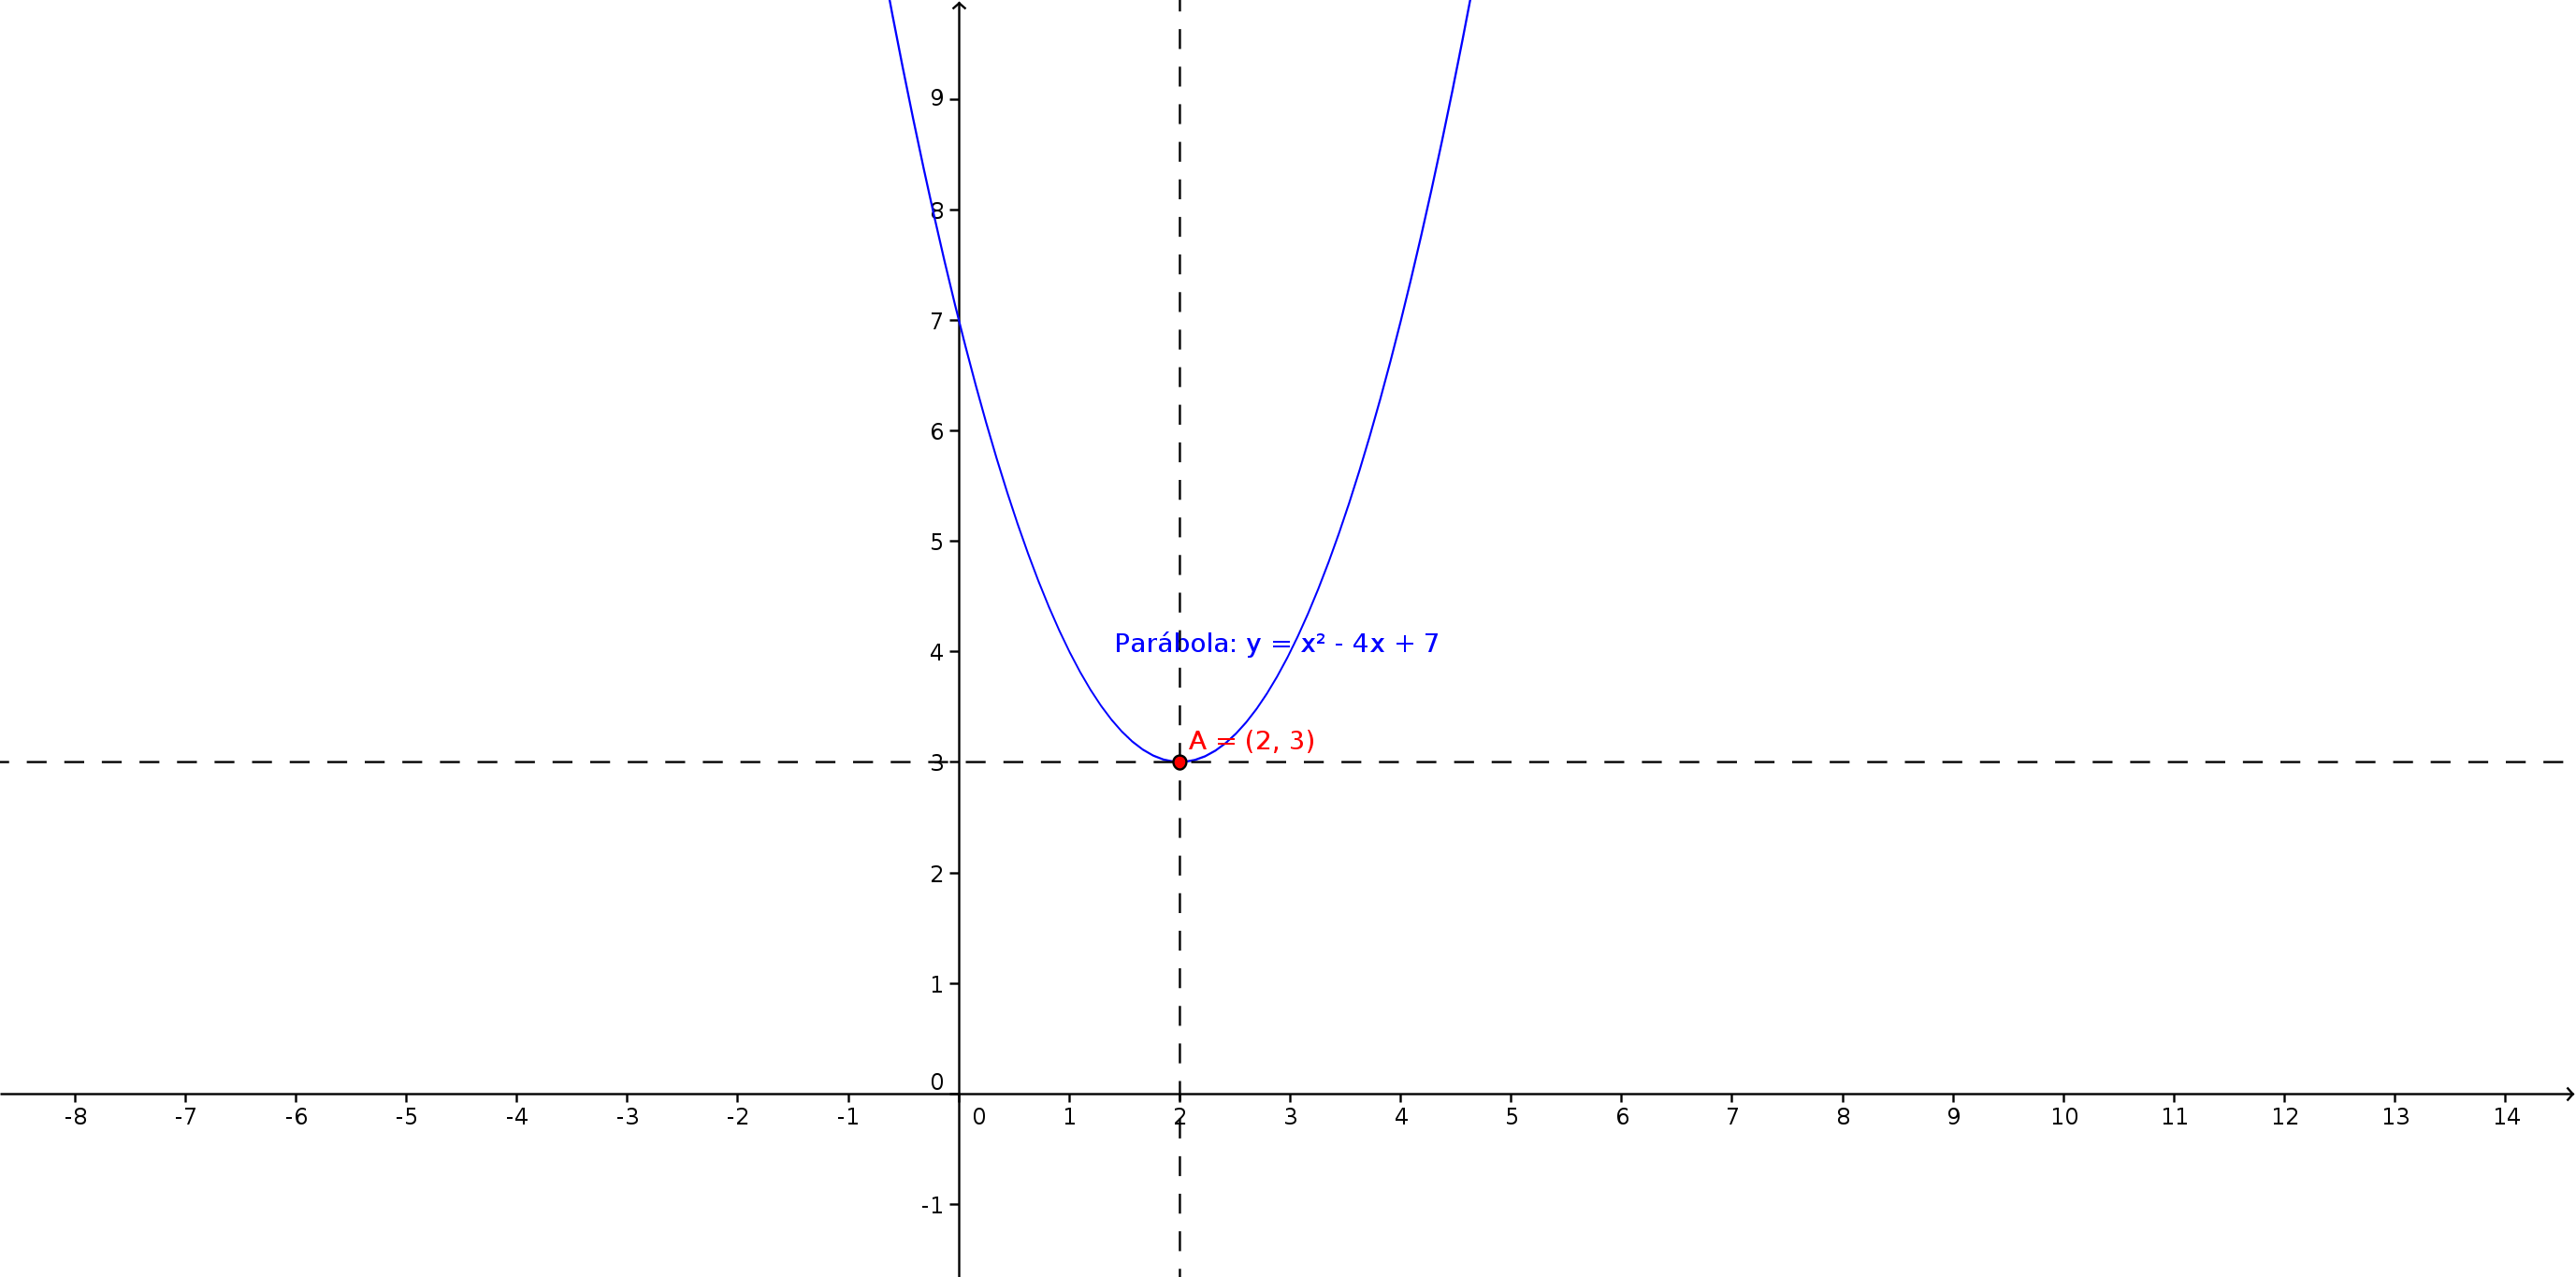
\includegraphics[height=5cm,keepaspectratio=true]{./precalculo/IM020401.png}
		% IM020401.png: 0x0 pixel, 300dpi, 0.00x0.00 cm, bb=
		\caption{$y=x^2-4x+7$}
		\label{fig:020401}
	\end{figure}
	


\subsection{Complemento de cuadrados}


	Cualquier funci\'on cuadrática se puede reescribir en la forma
	$$
	f(x)=a(x-h)^2+k,
	$$
	por el m\'etodo de \emph{complementos de cuadrado.}



	El punto $(h,k)$ se llama \emph{v\'ertice,} y corresponde al \emph{extremo} de la parábola
	$$
	y=a(x-h)^2+k.
	$$



	La f\'ormula para encontrar el v\'ertice de la parábola 
	$y=f(x)=ax^2+bx+c$ es
	$$\begin{cases}
		h=-\dfrac{b}{2a}\\
		k=f(h).
	\end{cases}
	$$ 



	Para completar el cuadrado, podemos usar el \emph{m\'etodo de divisi\'on sint\'etica:}
	\begin{center}
		\begin{tabular}{l|lll}
			$h$ & $a$ & $b$ & $c$\\
			& $\downarrow$ & $+ah$ & $\dots$\\\hline
			& $a$ & $\dots$ & $k$
		\end{tabular}
	\end{center}



	\begin{problema}
		Complete el cuadrado de
		$$y=x^2-4x+7.$$
	\end{problema}
	



	\begin{problema}
		Complete el cuadrádo de
		$$
		y=3x^2+30x+63.
		$$
	\end{problema}
	


\subsection{Intersecciones con los ejes}


	Las ra\'ices de un polinomio $p(x)$ son aquellos números reales $r$ tales que $p(r)=0.$



	Para encontrar las ra\'ices de una \emph{polinomio cuadrático}, necesitamos resolver la \emph{ecuaci\'on de segundo grado}
	$$
	a(x-h)^{2}+k=0.
	$$



	Si $r$ es una ra\'iz de $p(x)=a(x-h)^{2}+k,$ entonces la parábola $y=a(x-h)^{2}+k$ cruza al eje $x$ en el punto $(r,0).$




	\begin{observacion}
		Si bien $a,k>0$ o bien $a,k<0,$ entonces $a(x-h)^{2}+k>0$ y por tanto no existen ra\'ices. Por lo tanto, la parábola $y=a(x-h)^{2}+k$ \emph{nunca} cruza el eje $x.$ 
	\end{observacion}
	



	\begin{problema}
		Determine si existen ra\'ices de
		$$
		y=x^2-4x+7,
		$$ 
	\end{problema}
	



\subsection{Diferencia de cuadrados}


	Una identidad que es muy útil al momento de resolver ecuaciones es la \emph{diferencia de cuadrados}
	$$
	\left( a-b \right)\left( a+b \right)=a^{2}-b^{2}.
	$$



	Una ecuaci\'on de la forma 
	$$
	z^{2}-c^{2}=0
	$$
	se puede reescribir como
	$$
	\left( z-c \right)\left( z+c \right)=0...
	$$
	
	...en cuyo caso tenemos que $z-c=0$ o $z+c=0,$
	y por tanto las soluciones son
	$$
	z=\pm c.
	$$



	\begin{problema}
		Encuentre las ra\'ices de
		$$
		y=3x^2+30x+63.
		$$ 
	\end{problema}
	



	\begin{center}
		\includegraphics[height=5cm,keepaspectratio=true]{./precalculo/IM0301.png}
		% IM0301.png: 0x0 pixel, 300dpi, 0.00x0.00 cm, bb=
	\end{center}
	




\subsection{Ejemplos}


	\begin{problema} Resuelva las siguientes ecuaciones
		\begin{enumerate}
			\item $x^{2}-40=9$
			\item $2x^{2}-400=0$
			\item $x^{2}+36=9-2x^{2}$
		\end{enumerate}
		
	\end{problema}
	



	\begin{problema} Resuelva las siguientes ecuaciones
		\begin{enumerate}
			\item $\dfrac{x}{16}=\dfrac{4}{x}$
			\item $\dfrac{y^{2}}{3}=\dfrac{y^{2}}{6}+2$
		\end{enumerate}
		
	\end{problema}
	



	\begin{problema} Resuelva la siguiente ecuaci\'on
		$$
		\dfrac{1-2x}{3-x}=\dfrac{x-2}{3x-1}.
		$$
	\end{problema}
	



	\begin{problema} Resuelva la siguiente ecuaci\'on
		$$
		\dfrac{1}{2x-1}-\dfrac{1}{2x+1}=\dfrac{1}{4}.
		$$
	\end{problema}
	



	\begin{problema} Resuelva la siguiente ecuaci\'on
		$$
		x-\dfrac{2x}{x+1}=\dfrac{5}{x+1}-1.
		$$
	\end{problema}
	



	\begin{problema}
		\label{spi:exmp:16.2}
		Encuentre las ra\'ices de los siguientes polinomios
		\begin{enumerate}
			\item $7x^{2}-5x$
			\item $x^{2}-5x+6$
			\item $3x^{2}+2x-5$
			\item $x^{2}-4x+4$
		\end{enumerate}
		
	\end{problema}
	
	



	\begin{problema}
		\label{spi:exmp:16.3-}
		Encuentre las ra\'ices de los siguientes polinomios
		\begin{enumerate}
			\item $x^{2}-6x-2$
			\item $3x^2-5x+1$
			\item $4x^{2}-6x+3$   
		\end{enumerate}
		
	\end{problema}


\subsection{Factorizaci\'on}


	Si un polinomio $p(x)=ax^{2}+bx+c$ tiene ra\'ices $r_{1},r_{2}$ diferentes, entonces podemos factorizar de la siguiente manera
	$$
	p(x)=a(x-r_{1})\left( x-r_{2} \right).
	$$



	Si un polinomio $p(x)=ax^{2}+bx+c$ tiene una única ra\'z $r_{1}$, entonces podemos factorizar de la siguiente manera
	$$
	p(x)=a\left( x-r_{1} \right)^{2}.
	$$




	\begin{problema}
		\label{spi:exmp:16.2b}
		Factorice los siguientes polinomios
		\begin{enumerate}
			\item $7x^{2}-5x$
			\item $x^{2}-5x+6$
			\item $3x^{2}+2x-5$
			\item $x^{2}-4x+4$
		\end{enumerate}
		
	\end{problema}
	
	



	\begin{problema}
		\label{spi:exmp:16.3-b}
		Factorice los siguientes polinomios
		\begin{enumerate}
			\item $x^{2}-6x-2$
			\item $3x^2-5x+1$
			\item $4x^{2}-6x+3$   
		\end{enumerate}
		
	\end{problema}



\subsection{Aplicaciones}


	\begin{problema}
		\label{bron:exmp:16.21}
		Encuentre dos números positivos sabiendo que uno de ellos es igual al triple del otro más 5 y que el producto de ambos es igual a 68.
	\end{problema}
	



	\begin{problema}
		\label{bron:exmp:16.22}
		Encuentre un número sabiendo que la suma del triple del mismo con el doble de su rec\'iproco es igual a 5. 
	\end{problema}
	



	\begin{problema}
		\label{bron:exmp:16.23}
		Encuentre las dimensiones de un rectángulo cuto per\'imetro es de 50 pies y área es de 150 pies cuadrados. 
	\end{problema}



	\begin{problema}
		\label{bron:exmp:16.24}
		La hipotenusa de un triángulo es igual a 34 pulgadas. Encuentre las longitudes de los catetos sabiendo que uno de ellos es 14 pulgadas mayor que el otro.
	\end{problema}



	\begin{problema}
		\label{bron:exmp:16.25}
		Las dimensiones exteriores de un marco de fotograf\'ia son 12 por 15 pulgadas. Sabiendo que el ancho permanece constante, encuentre su valor a) cuando la superficie de la fotograf\'ia es de 88 pulgadas y b) cuando dicha superficie vale 100 pulgadas cuadradas. 
	\end{problema}



	\begin{problema}
		\label{bron:exmp:16.26}
		Un piloto realiza un vuelo de 600 millas. Sabiendo que si aumenta la velocidad en 40 millas/hora podr\'ia recorrer dicha distancia empleando 30 minutos menos, encuentre la velocidad promedio.  
	\end{problema}



	\begin{problema}
		\label{bron:exmp:16.27}
		Un comerciante compra determinado número de camisas por \$180 y las vende todas menos 6 con una ganancia de \$2 en cada camisa. Sabiendo que con el dinero recaudado en la venta podr\'ia haber comprado 30 camisas más que antes, calcule el precio de cada camisa.  
	\end{problema}



	\begin{problema}
		\label{bron:exmp:16.28}
		Dos operarios A y B juntos, realizan una tarea en 10 d\'ias. Trabajando por separado, A tardar\'ia 5 d\'ias más que B. Encuentre  el número de d\'ias que tardar\'ian en hacer la tarea trabajando cada no por s\'i s\'olo. 
	\end{problema}

